\chapter{Tecnologie}
La maggior parte delle tecnologie impiegate per lo sviluppo di questo progetto sono state definite nelle prime fasi di design, oltre che in fase di proposta dello stesso. Alcune librerie o specifici framework invece sono stati il risultato di scelte nate durante la fase di implementazione. Qui di seguito verranno descritte alcune tra le principali tecnologie utilizzate suddividendole tra quelle trasversali a tutto il progetto e quelle specifiche delle componenti di server, database e client.

\section{Tecnologie trasversali}

\subsection{NPM}
Node.js \cite{nodejsWikipedia} è un \emph{runtime system} multipiattaforma per l'esecuzione di codice JavaScript, costruito sul motore JavaScript V8 di Google Chrome.
Node.js dispone di una grande quantità di moduli scritti completamente in Javascript.
Essendo il progetto open-source è inoltre possibile per gli sviluppatori aggiungere i propri moduli in modo da renderli disponibili pubblicamente.

Il gestore di pacchetti predefinito per l'ambiente si chiama Node Package Manager.\emph{npm} può essere richiamato tramite linea di comando usando la seguente sintassi:
\begin{verbatim}
    npm <command> [args]
\end{verbatim}
Il comando base per ottenere un pacchetto è:
\begin{verbatim}
    npm install packet_name
\end{verbatim}
Tutte le dipendenze ed i conflitti vengono gestiti automaticamente \cite{npmDoc}. Grazie a Node è anche possibile per esempio creare un progetto React utilizzando il comando seguente:
\begin{verbatim}
    npx create-react-app project
\end{verbatim}
\emph{npx} è uno strumento integrato in npm in grado di eseguire pacchetti, anche se non sono ancora installati nel sistema.
Sarà poi possibile avviare il server di sviluppo utilizzando i seguenti comandi:
\begin{verbatim}
    cd project
    npm start
\end{verbatim}
L'interfaccia sarà poi visualizzabile all'indirizzo \emph{http://localhost:3000}.

\begin{figure}[H]
\centering

\includegraphics[width=0.3\textwidth]{img/logos/npm_logo.png}
\caption{npm logo}
\label{fig:npm}
\end{figure}

\subsection{Socket.io}
Socket.io è una libreria JavaScript che fornisce un servizio molto simile alle originali Web-Socket. Socket.io offre delle API JavaScript cross-browser che permettono la creazione di un canale di comunicazione full-duplex tra domini a bassa latenza tra il browser e il server web.

Socket.io tenta di utilizzare prima di tutto le WebSocket native. In caso fallisca (in caso di incompatibilità coi sistemi o a causa di altri problemi)
ricorrerà all'utilizzo di polling HTTP.

Socket.io è stato progettato per funzionare con tutti i browser moderni (97\% di compatibilità nel 2020) e in ambienti che non
supportano il protocollo WebSocket, ad esempio dietro proxy aziendali restrittivi.\\

Oltre alle funzionalità offerte da una tradizionale WebSocket, Socket.io offre inoltre le seguenti features:
\begin{itemize}
    \item reliability (switch a polling HTTP nel caso la connessione WebSocket non possa essere stabilita)
    \item riconnessione automatica
    \item buffering dei pacchetti
    \item acknowledgments
    \item broadcast a tutti i client o ad un sottoinsieme di essi (Room)
    \item multiplexing
\end{itemize}

\begin{figure}[H]
\centering

\includegraphics[width=0.4\textwidth]{img/logos/socketIO_logo.jpg}
\caption{Socket.io logo}
\label{fig:socketio}
\end{figure}

\subsection{Docker}
Docker è un sistema open-source tramite il quale è possibile automatizzare il processo di deployment di applicazioni all'interno di contenitori software.
Docker implementa API di alto livello per gestire \emph{container} che eseguono processi in ambienti isolati.

Utilizzando i container dunque le risorse possono essere isolate, i servizi limitati e i processi avviati in modo da avere una prospettiva completamente privata del sistema operativo, col loro proprio identificativo, file system e interfaccia di rete. Più container condividono lo stesso kernel, ma ciascuno di essi può essere costretto ad utilizzare una certa quantità di risorse, come la CPU, la memoria e l'I/O.

L'utilizzo di Docker per creare e gestire i container può semplificare la creazione di sistemi distribuiti, permettendo a diverse applicazioni o processi di lavorare in modo autonomo sulla stessa macchina fisica o su diverse macchine virtuali. Ciò consente di effettuare il deployment di nuovi nodi solo quando necessario.

Al fine di creare un container Docker sarà necessario specificare un \emph{Dockerfile} per ogni servizio erogato. 
Similmente ai gitignore per il versioning git, è possibile definire dei \emph{dockerignore} per segnalare a docker quali file ignorare durante la copia dei file all'interno del container. Per gestire invece applicazioni composte da più servizi sarà possibile utilizzare \emph{Docker Compose}, uno strumento che permette con un solo comando di avviare un intero sistema isolato gestendo nello specifico dipendenze tra servizi, volumi e reti.

\begin{figure}[H]
\centering

\includegraphics[width=0.5\textwidth]{img/logos/docker_logo.png}
\caption{Docker logo}
\label{fig:docker}
\end{figure}

\section{Tecnologie Server}
\subsection{Node.js}
Node.js \cite{nodejsWikipedia} è un \emph{runtime system} multipiattaforma per l'esecuzione di codice JavaScript, costruito sul motore JavaScript V8 di Google Chrome, progettato per creare applicazioni di rete scalabili. Grazie al suo funzionamento molte connessioni possono essere gestite contemporaneamente, per ognuna delle quali verrà invocata una callback, rendendo Node attivo solo al momento necessario.\\

Node.js implementa un'architettura event-driven, facendo dunque affidamento su un event loop. Non esiste alcuna chiamata per avviare il ciclo: Node.js entra semplicemente nel ciclo degli eventi dopo aver eseguito lo script di input e, analogamente, esce dal ciclo di eventi quando non ci sono più callback da eseguire. Questo comportamento è simile a JavaScript in browser: il ciclo degli eventi è nascosto all'utente.
Per natura dell'event loop, Node è single-threaded, ma è possibile, su necessità, effettuare delle fork per sfruttare al meglio i core offerti dalla macchina creando nuovi thread.

\begin{figure}[H]
\centering

\includegraphics[width=0.3\textwidth]{img/logos/nodejs_logo.png}
\caption{Node.js logo}
\label{fig:nodejs}
\end{figure}

\subsection{Express}
Express è un framework web per Node.js che semplifica lo sviluppo di applicazioni web e API. Fornisce una serie di funzionalità per gestire richieste HTTP, definire \emph{rotte}, elaborare dati di input e gestire le risposte. Express è estremamente flessibile e leggero, consentendo agli sviluppatori di creare rapidamente applicazioni web scalabili e con ottime prestazioni.

Una delle caratteristiche principali di Express è il concetto di \emph{middleware}, ovvero funzioni che possono essere eseguite prima, durante o dopo il processo di gestione delle richieste. Questo consente agli sviluppatori di rendere modulare il codice e aggiungere facilmente funzionalità come autenticazione e gestione degli errori.

Express segue il paradigma di programmazione event-driven di Node.js e si integra perfettamente con esso. Può essere utilizzato insieme ad altri moduli Node.js per gestire aspetti specifici delle applicazioni web, come la gestione delle sessioni utente o la connessione al database.

Grazie alla sua vasta adozione nella comunità Node.js, Express ha una vasta gamma di plugin e middleware disponibili, che permettono agli sviluppatori di estendere facilmente le funzionalità base del framework per adattarsi alle esigenze specifiche del progetto.

In sintesi, Express è un potente framework per lo sviluppo di applicazioni web con Node.js, che offre una combinazione di flessibilità, prestazioni e facilità d'uso.

\begin{figure}[H]
\centering

\includegraphics[width=0.4\textwidth]{img/logos/expressjs_logo.png}
\caption{Express logo}
\label{fig:express}
\end{figure}

\subsection{Mongoose}
Mongoose è una libreria per Node.js che permette di creare degli \emph{Schema} per rappresentare i dati da archiviare nel sistema.
Ogni Schema è associato ad una collezione nel Database di MongoDB.
Mongoose viene utilizzato per la creazione del proprio model, essendo possibile creare delle istanze dallo Schema attraverso delle \emph{Factory} ed utilizzarli come dei semplici oggetti Javascript.
Oltre ad offrire metodi aggiuntivi già pronti per salvare i dati all'interno del database è possibile creare funzioni che solo oggetti appartenenti ad un relativo schema possono richiamare, rendendo la modellazione simile all'object-oriented.\\

\begin{figure}[H]
\centering

\includegraphics[width=0.3\textwidth]{img/logos/mongoose_logo.png}
\caption{Mongoose logo}
\label{fig:mongoose}
\end{figure}

\section{Tecnologie Database}
\subsection{MongoDB}
MongoDB è un DBMS NoSQL, cioè non utilizza un meccanismo di persistenza relazionale come un tradizionale SQL.
Il modello NoSQL non è unico e può dunque utilizzare varie strutture dati per sostituire le tabelle con campi uniformi utilizzate in SQL.

In particolare MongoDB utilizza un modello orientato al documento, dove le informazioni sono memorizzate in una struttura gerarchica ad albero ed un qualsiasi numero di campi con qualsiasi lunghezza può essere aggiunto. I campi a loro volta possono contenere aggregati di dati composti da più elementi o da strutture annidate.

I DBMS orientati al documento offrono alcuni vantaggi, specialmente in ambito web, rispetto ai tradizionali RDBMS. Si ottengono maggior flessibilità dei dati, utile per avere meno rigidità in fase di sviluppo o, in generale, per scenari in cui i dati memorizzati non sono sempre uniformi, e una maggior facilità nella trasposizione in strutture dati nel codice in quanto i JSON, utilizzati da MongoDB, trovano una corrispondenza uno ad uno con esse. Il trade-off nell'avere una struttura meno rigida è però il rischio di duplicazione di dati ed inconsistenze, per cui è richiesta al progettista una maggiore cautela nella manipolazione di dati.

\begin{figure}[H]
\centering

\includegraphics[width=0.3\textwidth]{img/logos/mongo_logo.png}
\caption{MongoDB logo}
\label{fig:mongodb}
\end{figure}


\section{Tecnologie Client}

\subsection{React.js}
React è un framework open-source che permette di implementare applicazioni web seguendo i principi della programmazione ad oggetti. In modo particolare risulta essenziale descrivere tre concetti chiave:
\begin{itemize}
    \item \textbf{JSX:} è un'estensione della sintassi di JavaScript.\cite{introduzione_jsx_react} Permette di unire gli aspetti di html come linguaggio di template agli aspetti di JavaScript come linguaggio di scripting in una forma che ne aumenta semplicità e leggibilità. Gli elementi JSX vengono utilizzati nelle definizioni delle funzioni di rendering semplificando la costruzione della UI. Attraverso JSX si può richiamare un componente React tramite con un meccanismo analogo ai tag in html.
    \item \textbf{Componenti:} attraverso un componente\cite{componente_react} si va a definire quella che risulta essere a tutti gli effetti una classe. Il componente, definito da uno o più costruttori, contiene uno stato, il quale verrà mantenuto, ed eventualmente aggiornato, durante tutto il ciclo di vita dello stesso. È possibile ricevere dati ed istruzioni da altri componenti attraverso le props.
    \item \textbf{Stato:} è un insieme di proprietà di un componente.\cite{state_e_lifecycle_react} Queste proprietà possono variare a seguito dell'interazione con altri componenti o come azione del componente stesso nel caso esso esegua delle azioni a cadenza temporale. In React lo stato risulta inoltre fondamentale ai fini di ottenere un aggiornamento delle interfacce performante. Ogni componente React deve obbligatoriamente definire una funzione \emph{render()}. Attraverso di essa verrà ritornato il contenuto da renderizzare. React cambierà il contenuto della UI, utilizzando quindi risorse, solamente quando vi saranno delle modifiche nel contenuto ritornato dalla funzione \emph{render()}. Utilizzando dunque le proprietà che definiscono lo stato del componente all'interno di questa funzione sarà possibile ridurre al minimo il numero di volte in cui l'applicazione verrà renderizzata, riflettendo i cambiamenti di stato del componente.    
\end{itemize}

React infine introduce anche i componenti funzione, che di fatto svolgono la stessa funzione dei componenti precedentemente descritti, ma con una sintassi più concisa.

\begin{figure}[H]
\centering

\includegraphics[width=0.2\textwidth]{img/logos/react_logo.png}
\caption{React logo}
\label{fig:react}
\end{figure}


\subsection{Redux}

Redux \cite{caratteristiche_redux} è un \emph{contenitore di stato} per applicazioni JavaScript. Gode di quattro caratteristiche fondamentali per progetti portata medio-grande:
\begin{itemize}
  \item \textbf{Deterministico:} aspetto fondamentale nelle applicazioni web di ogni genere è il determinismo. L'oneroso compito di far collaborare tutti i componenti al fine di ottenere un comportamento predicibile viene largamente semplificato dall'utilizzo di questo framework.
  \item \textbf{Centralizzato:} avere stato e logica centralizzati permette di ottenere rapidamente delle feature di fondamentale importanza, come funzioni di "annulla" e "ripeti" che permettono di muoversi agilmente tra lo storico degli stati. Un approccio centralizzato garantisce inoltre una consistenza maggiore dei dati, rendendo possibile modificarli solamente attraverso specifiche funzioni, le azioni, create durante la definizione della struttura dati.
  \item \textbf{Debug oriented:} attraverso semplici plugin browser come Redux DevTools risulta immediato il debug dell'applicazione. Attraverso questi tool si ottiene una visione completa dello stato dei dati e della sua evoluzione nel tempo, riuscendo ad identificare con precisione quando e soprattutto perché lo stato abbia subito delle modifiche.
  \item \textbf{Flessibile:} Redux funziona con ogni layer di UI e, essendo ormai uno strumento consolidato, dispone di un solido supporto e una vasta proposta di plugin e pacchetti aggiuntivi per ogni esigenza.
\end{itemize}
Per comprendere come queste caratteristiche si concretizzino risulta fondamentale comprendere tre concetti chiave nella struttura di Redux:
\begin{itemize}
  \item \textbf{Store:} è un oggetto che contiene l'intera struttura ad albero dello stato.\cite{store_redux} Fornisce metodi per la lettura dello stato corrente.
  \item \textbf{Reducer:} definiscono la struttura dello store.\cite{reducer_redux} Vi possono essere più reducer all'interno di una stessa applicazione, al fine di meglio suddividere lo stato.
  \item \textbf{Azioni:} permettono di modificare il contenuto dello store.\cite{azioni_redux} Essendo queste l'unico modo per alterare lo stato attuale, qualsiasi componente che voglia agire sullo stato deve passare per le azioni definite.
\end{itemize}
Ci sono alcune motivazioni che portano alla scelta di utilizzare questo strumento in aggiunta allo stato messo a disposizione da React. Quest'ultimo pur essendo uno strumento molto potente, pone davanti a delle limitazioni.

Non è raro che più componenti all'interno dell'applicazione debbano fare riferimento allo stesso dato, per cui la presenza di uno stato comune evita di dover implementare meccanismi ad hoc di sincronia tra gli stati dei due componenti. Lo stato di ogni componente, attraverso strumenti preesistenti, sarà dunque sincronizzato con la struttura principale.

React inoltre, data la sua natura orientata alla programmazione reattiva, incoraggia la propagazione dell'informazione solo in una direzione: da un componente padre verso un componente figlio. La presenza delle azioni Redux risolve questo problema in quanto ogni cambiamento apportato allo stato Redux si rifletterà su tutti i componenti React che utilizzano quel particolare dato, in maniera trasparente nei confronti della loro gerarchia.

\begin{figure}[H]
\centering
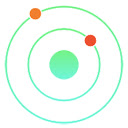
\includegraphics[width=0.3\textwidth]{img/logos/redux_devtool.jpg}
\caption{Redux logo}
\label{fig:redux}
\end{figure}

\subsection{Bootstrap}

Bootstrap è stato creato nel 2010, tramite Twitter, da @mdo and @fat. È rapidamente diventato il framework più popolare per il front-end a livello mondiale. Con le prime release della versione 2 vennero introdotti i primi fogli di stile per aggiungere funzionalità riguardanti il design responsive. Con l'uscita della versione 3 l'intera libreria è stata ripensata e riscritta per offrire supporto al design responsive con un approccio mobile-first. La versione 4 di Bootstrap, ovvero quella attuale, ha subito infine due principali cambiamenti nella sua architettura:
\begin{itemize}
    \item una migrazione a Sass, un'estensione del linguaggio CSS che permette l'uso di variabili e di funzioni,
    \item l'uso di CSS flexbox, ovvero contenitori per elementi.
\end{itemize}

Come detto in precedenza, Bootstrap adotta un approcio mobile-first. L'assunzione di base è che la maggior parte dei visitatori utilizzeranno uno smartphone a causa del sempre più crescente utilizzo di questo tipo di dispositivi. L'utilizzo continuo di media query è alla base di ogni layout creato utilizzando Bootstrap \cite{bootstrap}. Moltissime classi offerte utilizzano i cosiddetti breakpoints. Si tratta di meccanismi che permettono di nascondere, mostrare o modificare il comportamento degli elementi a cui vengono applicate in base alla risoluzione dello schermo del visitatore.
Bootstrap mette a disposizione i seguenti breakpoints:
\begin{minted}{css}
// Small devices (landscape phones, 576px and up) KEYWORD:sm
    @media (min-width: 576px) { ... }
    
// Medium devices (tablets, 768px and up) KEYWORD:md
    @media (min-width: 768px) { ... }
    
// Large devices (desktops, 992px and up) KEYWORD:lg
    @media (min-width: 992px) { ... }
    
// Extra large devices (large desktops, 1200px and up) KEYWORD:xl
    @media (min-width: 1200px) { ... } 
\end{minted}
Segue un rapido esempio per l'uso dei breakpoints. Per la gestione dei margini e del padding Bootstrap mette a disposizione le classi di tipo 
\begin{verbatim}
    {property}{sides}-{breakpoint}-{size}
\end{verbatim}
\begin{itemize}
    \item \textbf{property:} assume valore\textbf{m} se si vuole aggiungere un margine, \textbf{p} se si vuole aggiungere del padding.
    \item \textbf{sides:} assume valore\textbf{t} per top, \textbf{b} per bottom, \textbf{r} per right, \textbf{l} per left, \textbf{x} per right e left, \textbf{y} per top e bottom.
    \item \textbf{breakpoints:} se omesso, la classe funziona su qualsiasi tipo di schermo, anche i più piccoli, altrimenti funziona solo sugli schermi più grandi anche solo di un pixel del breakpoint specificato.
    \item \textbf{size:} Bootstrap non utilizza valori statici per specificare di quanto deve essere il padding o il margine. Il valore che può assumere size va da 0 a 5, e sono valori che indicano quando deve essere grande il moltiplicatore che gestisce lo spazio. \textbf{0} significa nessun padding o margine.
\end{itemize}
Seguendo queste indicazioni se si desidera applicare un piccolo margine a destra ad un determinato elemento solo se visualizzato su uno schermo con larghezza maggiore di 992px, le classi che l'elemento dovrà assumere saranno \emph{mr-0 mr-lg-2}. Appartenere alla prima classe, \emph{mr-0}, significa nessun margine a destra su qualsiasi tipo di schermo, mentre per la seconda, \emph{mr-lg-2}, vuol dire invece avere un margine a destra con proporzione 2 solo su schermi più grandi di 992px. Combinando insieme le due classi otteniamo un margine che varia in maniera reattiva alla dimensione dello schermo\cite{bootstrapDoc}.

\begin{figure}[H]
\centering

\includegraphics[width=0.3\textwidth]{img/logos/bootstrap_logo.png}
\caption{Bootstrap logo}
\label{fig:bootstrap}
\end{figure}


\subsection{PeerJS}

PeerJS è una libreria JavaScript open-source nata per semplificare la creazione di applicazioni \emph{peer-to-peer} in modo trasparente e affidabile. Utilizzando WebRTC, ovvero Web Real-Time Communication, PeerJS permette di stabilire connessioni dirette tra i browser senza la necessità di server intermediari. Questo approccio decentralizzato riduce la latenza e il carico di lavoro sul server, migliorando l'efficienza e la scalabilità delle applicazioni P2P.

Sfruttando PeerJS è possibile creare e gestire connessioni P2P in modo semplice, avendo a disposizione API intuitive per aprire, accettare e gestire le connessioni. La libreria gestisce automaticamente aspetti complessi come il \emph{signaling} e il trasporto dei dati attraverso i peer connessi, consentendo di concentrarsi maggiormente sulla logica dell'applicazione anziché sulle complessità della comunicazione in tempo reale.

Tra le funzionalità offerte utili per la creazione di questo tipo di applicazioni le principali sono la trasmissione di dati in tempo reale, la condivisione di file e la comunicazione audio/video. Inoltre, essendo basato su WebRTC, PeerJS è compatibile con la maggior parte dei browser moderni e fornisce quindi una soluzione sicura e di facile utilizzo.

Per poter connettere i peer l'un l'altro è necessario però avere un server che svolga il compito di \emph{connection broker}, per cui non riceverà nessun dato della rete P2P. Per quanto riguarda l'hosting del server, PeerJS offre due opzioni:
\begin{itemize}
    \item utilizzare il PeerServer Cloud fornito direttamente dagli sviluppatori della libreria, che è una versione cloud-hosted gratuita del PeerServer ufficiale. Questa opzione è conveniente per chi non ha specifiche necessità e preferisce una soluzione facile da implementare,
    \item eseguire il proprio PeerServer, utilizzando il codice sorgente open-source scritto in Node.js disponibile online. Questa opzione offre maggiore controllo e flessibilità, ma richiede competenze tecniche per l'installazione e la configurazione.
\end{itemize}

\begin{figure}[H]
\centering

\includegraphics[width=0.4\textwidth]{img/logos/peerjs_logo.png}
\caption{PeerJS logo}
\label{fig:peerjs}
\end{figure}